\chapter{基于深度学习的辐射源未知分类识别}

\section{引言}


在跟踪发达国家研究进展的基础上,国内也开始加紧研发可装备于军方的 SEI 系统,以逐步缩小与发达国家在技术实用方面的差距。但总体来说,我国在该方面的研究还赶不上美英等发达国家,除了缺乏深层次且系统化的理论分析研究外,更缺乏成熟的工程化系统实践和实际装备,因而迫切需要加快在该领域的理论研究和应用步伐。本文综合雷达信号处理、深度学习等多学科理论,重点围绕在复杂电磁环境下不同辐射源的个体识别所面临的识别能力差等问题与挑战,提出合理的雷达脉内细微特征模型,结合深度学习的理论与方法,解决传统辐射源识别方法的局限性,为雷达辐射源识别提供理论支撑于技术指导

Open Set目标识别系统必须可以准确的处理下面三种类型的数据类:
\begin{itemize}
	\item 已知的(目标)类,被标记为正面训练样本的数据。
	\item 已知的未知(非目标)类,被标记为负面训练样本的数据。
	\item 未知的未知(非目标)类,在训练样本中不存在的类别的数据。
\end{itemize}

国内外对于Open Set的识别也早有研究,Simonson 提出了一种称作probabilistic fusion (PF)的利用统计的方法来进行Open Set识别,其主要通过合并来自不同数据源的证据得到一个统计测试模型,根据此模型的分布来对于类别进行判断。Scheirer等人提出了一种通过分析后验数据得分来进行类型判断的方法。

% 详细分析不同辐射源雷达信号的差别,研究不同雷达的信号建模过程以及据此获取雷达信号的基本特征;对雷达有意调制和无意调制这两种脉内调制形式进行建模,综合分析其对应的各种特征(瞬时自相关、相位差分法、模糊函数等);综合考虑各种脉内细微特征,建立基于深度学习的分类结构;结合大量数据,对结构进行验证和调整;基于实际数据,对算法的各种特性进行验证。

\section{辐射源信号分析}

对于辐射源信号的处理,本文主要考虑两方面:信号预处理、特征提取优化。

在信号预处理方面,首先需要剔除无用和错误的数据。然后将信号进行分选,其主要是从随机交叠的脉冲信号流中分离出各个雷达的脉冲信号并选出有用信号。其实质是去交叠、去交错,所利用的是同一部雷达信号参数的相关性和不同雷达信号参数的差异性。

在特征提取优化方面,合理的特征是分类识别的基础。本文以模糊函数为平台,分析提取其切片特征。

\subsection{模糊函数}

模糊函数不仅能描述雷达信号的分辨特性和模糊度,还能描述由雷达信号所决定的测量精度和杂波抑制特性等,并根据这种雷达无意调制产生的信号脉内细微特征来进行分类所需的特征。对于信号$x(t)$,其瞬时自相关函数为$R_x(t,\tau)=x(t+\tau/2)x^{*}(t-\tau/2)$,其中$\tau$为时延,模糊函数的定义为,
\begin{equation}
A(\tau,\nu) = \int_{-\infty}^{+\infty}R_x(t,\tau)e^{j2\pi\nu t}dt
\end{equation}
即$R_x(t,\tau)$关于时间$t$的傅里叶反变换。由于在实际中发射机自身存在相位噪声以及各类杂散输出,故可以区分出型号、参数均相同的辐射源,通过模糊函数在时延和频偏这二维上的变换,可以多角度的刻画出无意调制对于发射信号的影响。

为了方便在数字信号中使用,上式可以经过变换等价于下面的形式:
\begin{equation}
A(\tau,\nu) = \int_{0}^{\tau}x(t)x^{*}(t+\tau)e^{j2\pi\nu t}dt
\end{equation}
对信号均匀采样,即对接收信号和参考信号离散化后,上式可以表示为:
\begin{equation}
A(\tau_l,\nu_m) = A(l, m) = \sum_{n = 0}^{N-1}x(n)x^{*}(n+l)e^{\frac{j2\pi m n}{N}}	
\end{equation}
其中,$\tau_l=l/f_s$,$\nu_m=mf_s/N$。

\begin{figure}
	\centering
	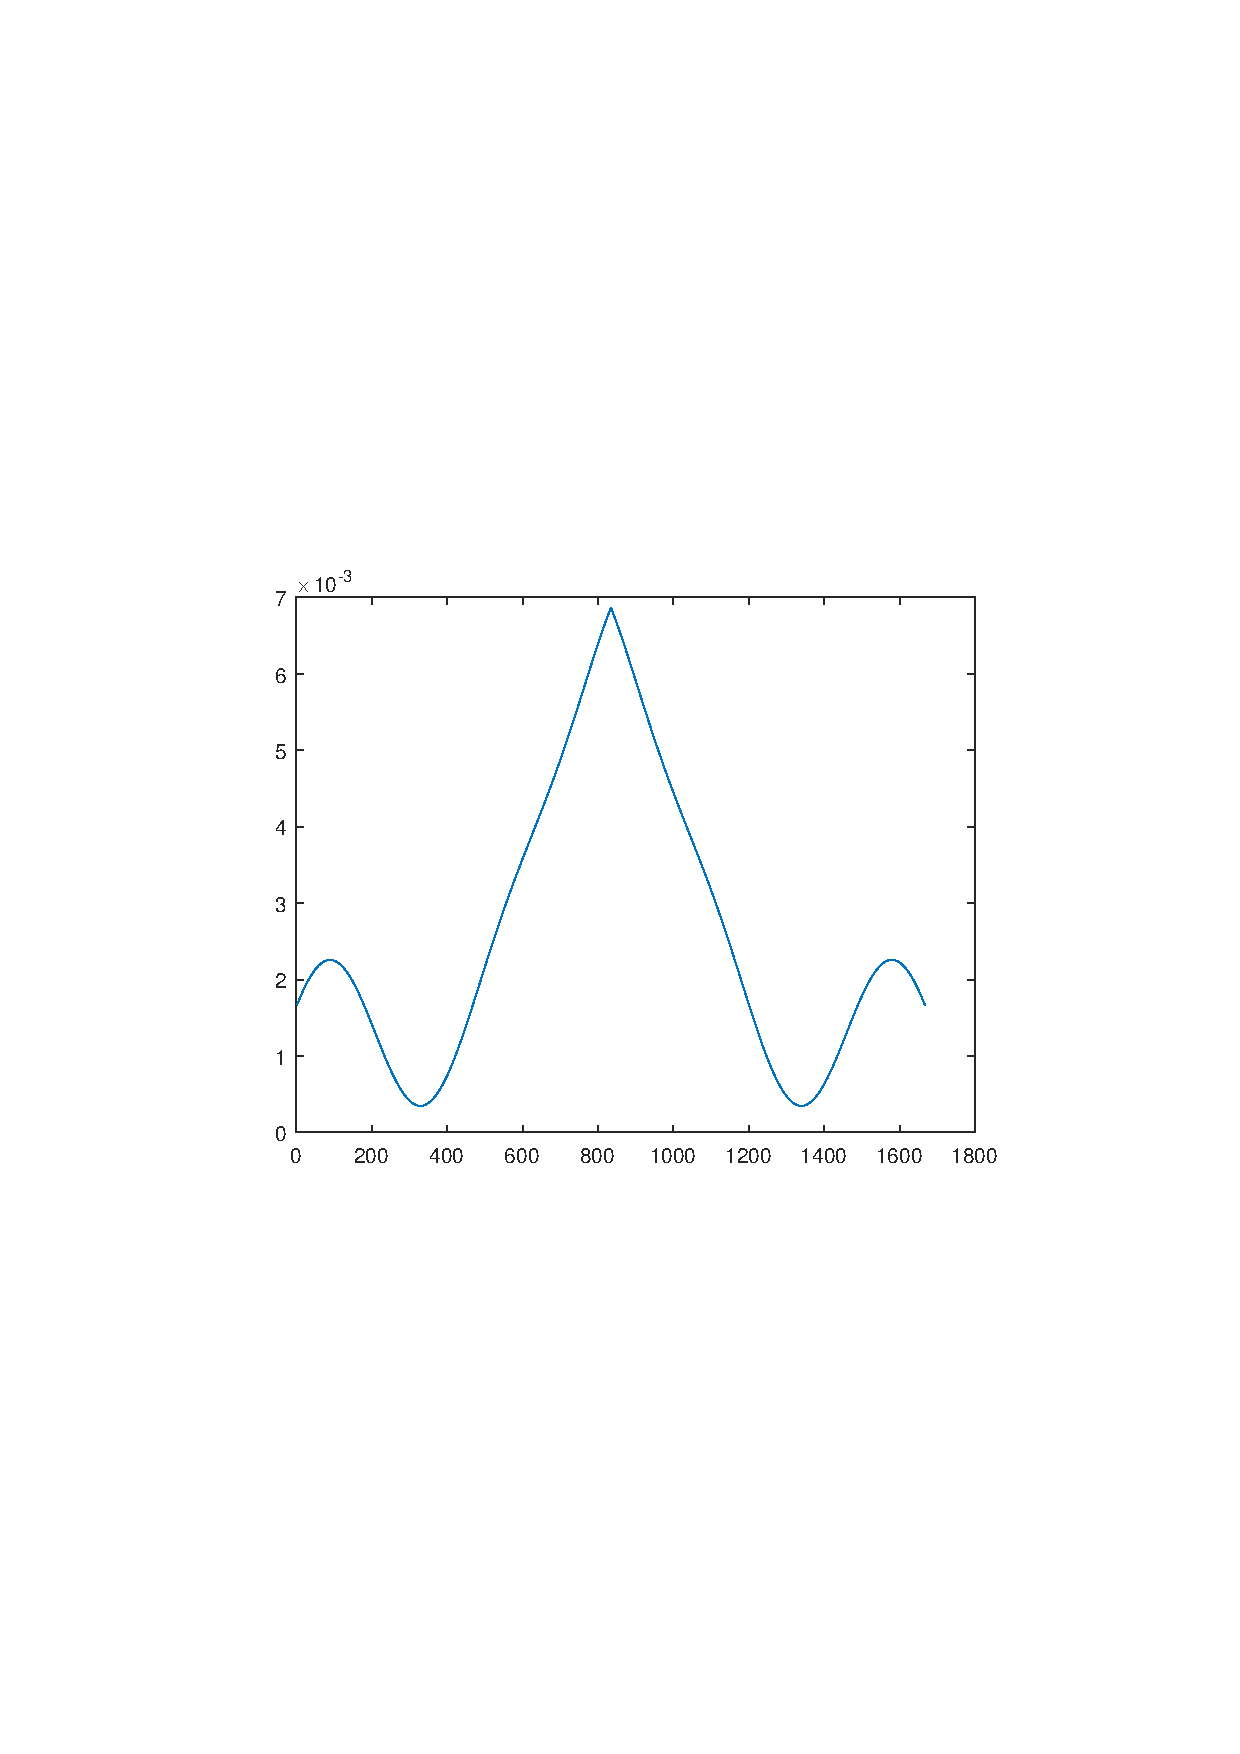
\includegraphics{figures/af.pdf}
	\caption{模糊函数切片图}
\end{figure}

\section{Open Set 分类器设计}

此部分主要解决的问题是当得到一个新的测试样本,如果该样本不属于已经经过训练的分类,那么传统的神经网络模型会将该样本指派给与其最相似的一个类别,此种情况对于一个Open Set识别系统,也即类似于辐射源识别系统这种具有较多尚未经过训练的样本的一个数据集,首先这会导致其识别率下降,另一方面是由于对于未知的辐射源无法很好的确定,无法很好的完成预警等任务。国内外学者对于该问题的研究主要分为下面两个思路:

\begin{itemize}
	\item 在训练集中添加一个“未知”类别,利用不同的来自非已知类别的数据作为训练样本对该类别进行训练,然后对于所有的输入数据进行类别的识别,对于识别结果为该类别的数据作为未知分类。然而该思路最大的问题是我们无法得到所有可能的未知类别的样本来进行训练,具有一定的局限性。
	
	\item 针对于多分类使用的softmax函数,可以设立阈值或者对于该识别结果进行一个评价(例如与已知类别数据的一个“距离”)等进行分辨出未知的分类。
\end{itemize}

针对于该问题,我们基于思路2的想法设计了一个基于meta-recognition的可以识别未知辐射源的深度神经网络。首先是创建一个深度卷积神经网络分类器,该分类器的输出为该训练样本属于各个类别的概率,我们然后将此类别作为一个输入,输入到我们的meta-recognition中,这里我们设计一个支持向量机分类器作为meta-recognition,然后从该meta-recognition会进行判断该输入是否为一个未知分类。

\begin{figure}
	\centering
	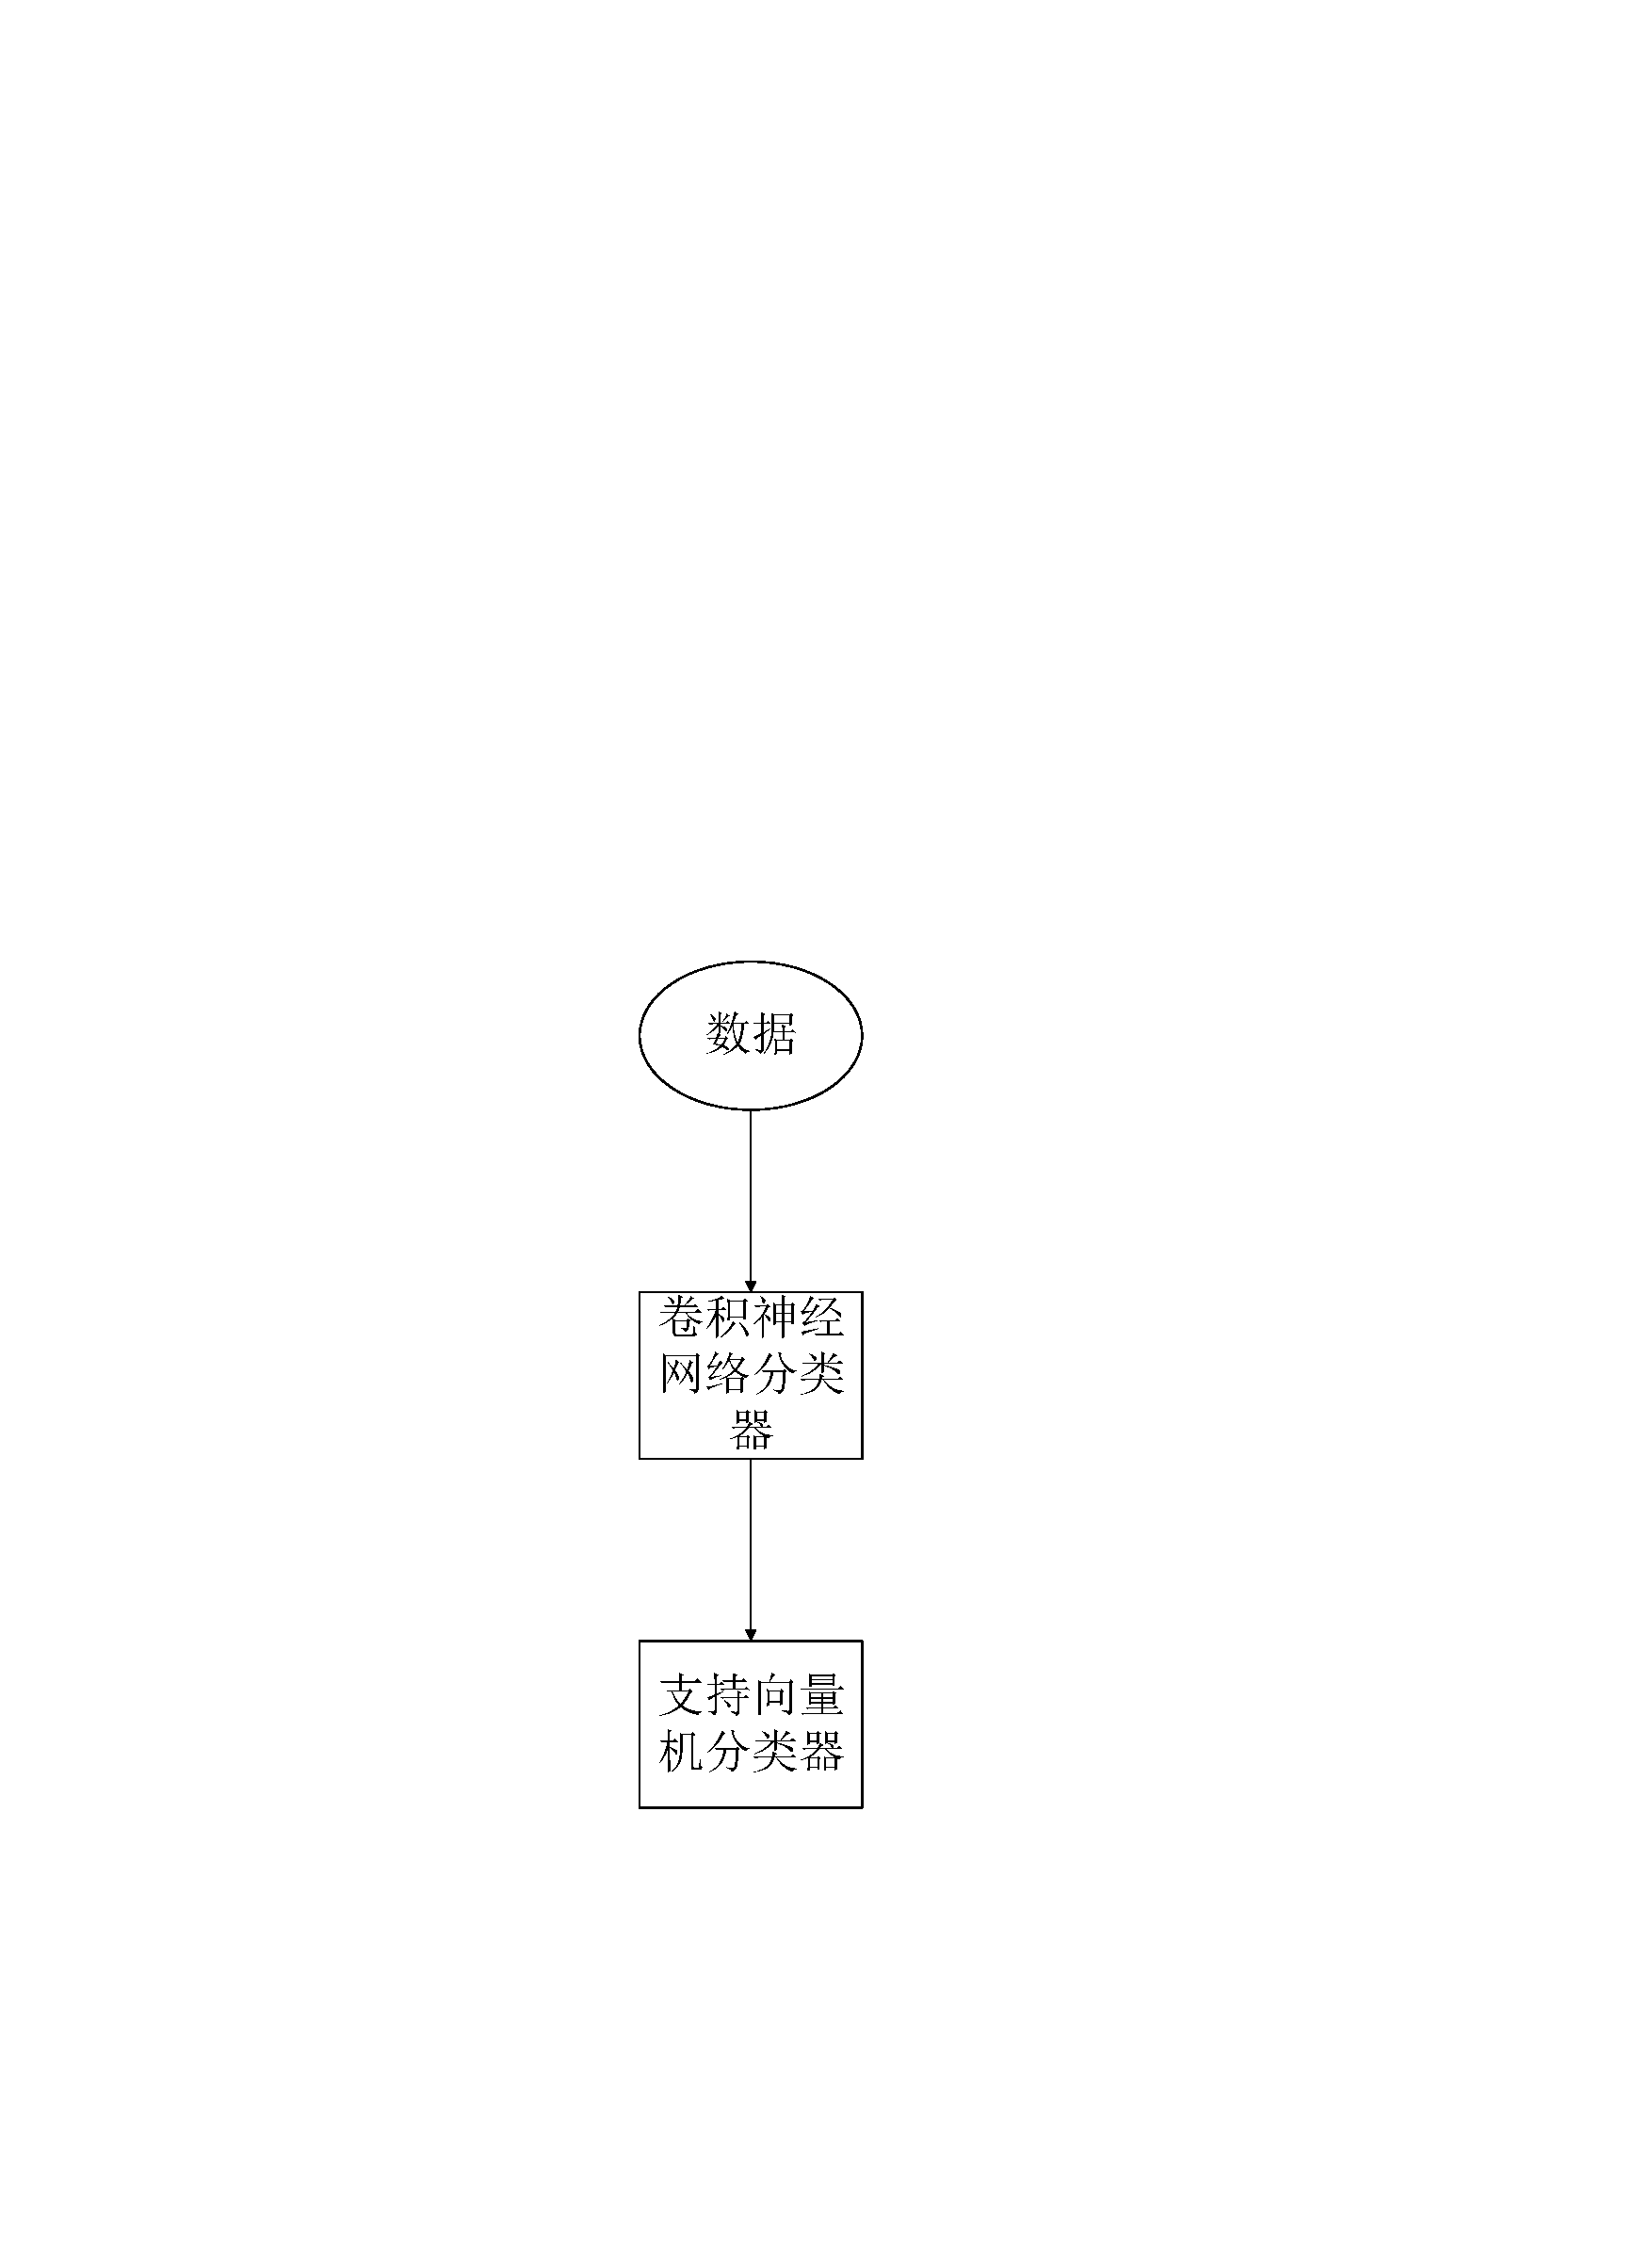
\includegraphics{figures/frame.pdf}
	\caption{分类器设计结构图}
\end{figure}


\subsection{深度卷积神经网络分类器设计}

在分类器设计方面,本文设计利用卷积神经网络的分类器。典型的卷积神经网络由深层结构堆叠在一起的多个不同的层组成:输入层,多组卷积和池化层,有限数量的完全连接的隐藏层,以及输出层。其中最主要的部分为卷积层。其利用输入数据中的局部结构,将整个输入空间划分成很小的隐藏单元。将各个隐藏单元的权重构建得到的卷积核作用于整个输入空间,从而得到特征向量。利用这种机制,我们不仅大大减少了参数数量同时提高了数据的平移不变性。据辐射源信号的实际数据以及其反映出来的特性,构建了基本的具有 13 层的卷积神经网络,每层具有多个特征向量,每个特征向量具有多个神经元,并且每个特征向量来自于一种卷积核所提取输入的一种特征。主要过程为对于输入的辐射源信号,进行多次的卷积、池化操作,进行再次特征提取,然后通过BP网络进行训练。
\begin{figure}
	\centering
	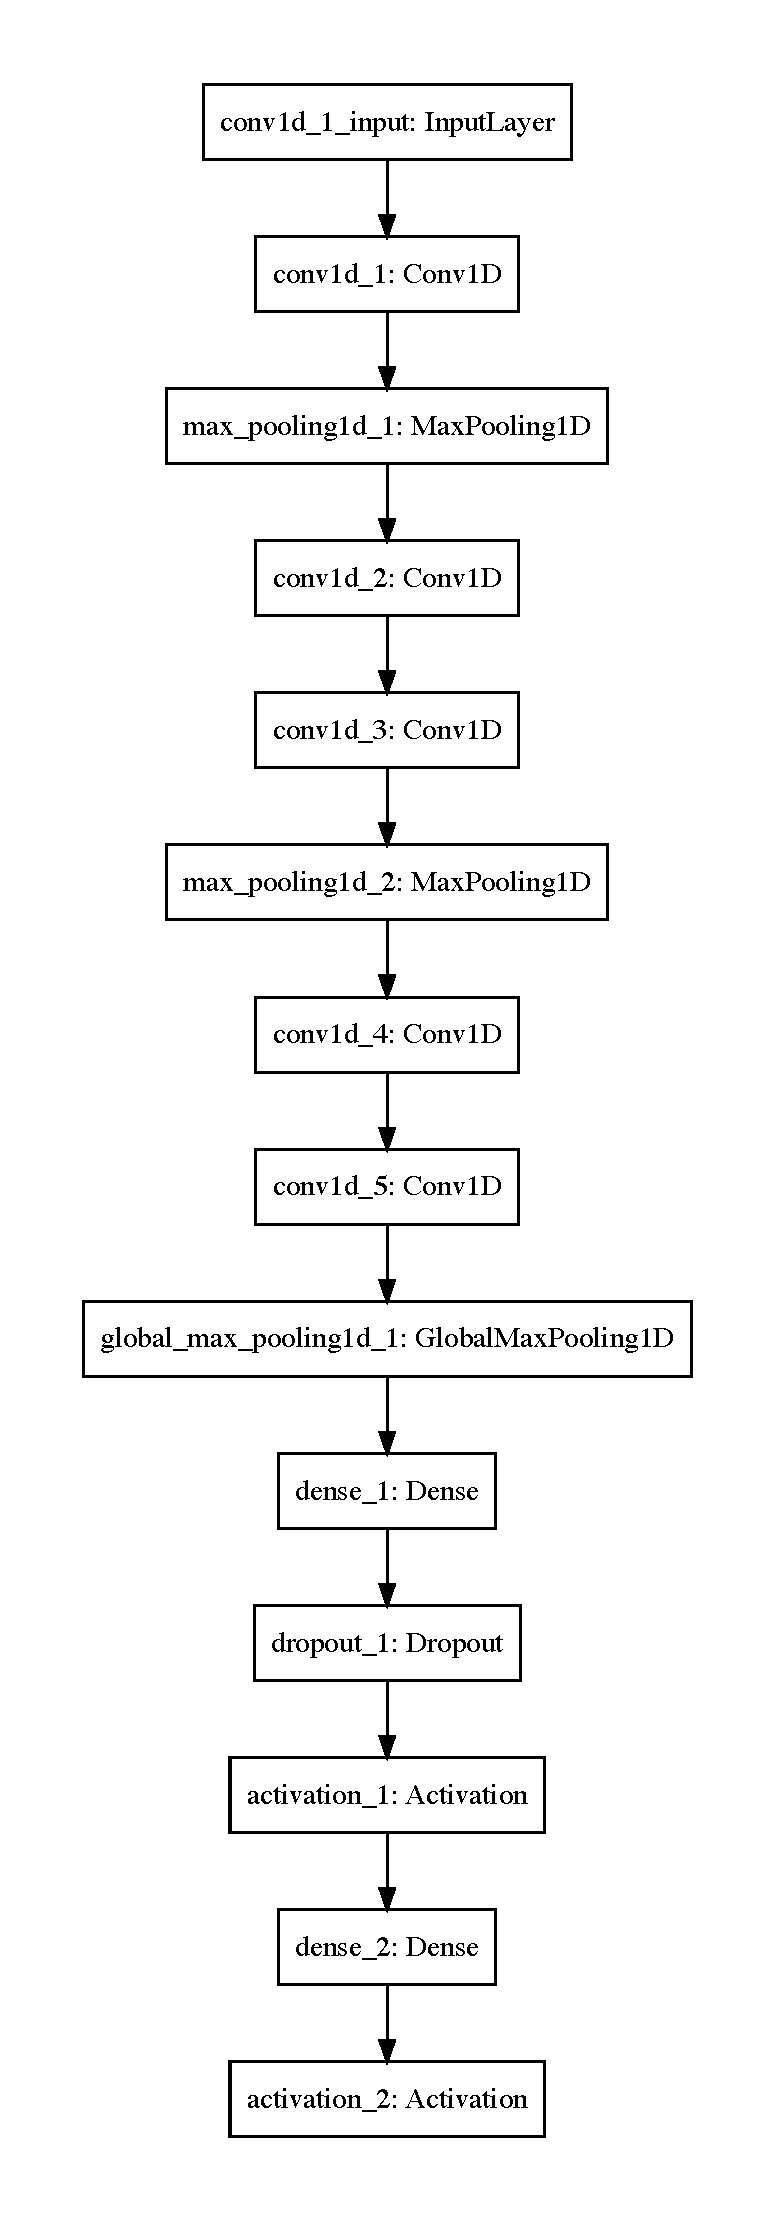
\includegraphics{figures/cnn.pdf}
	\caption{深度卷积神经网络框架图}
\end{figure}

\begin{figure}
	\centering
	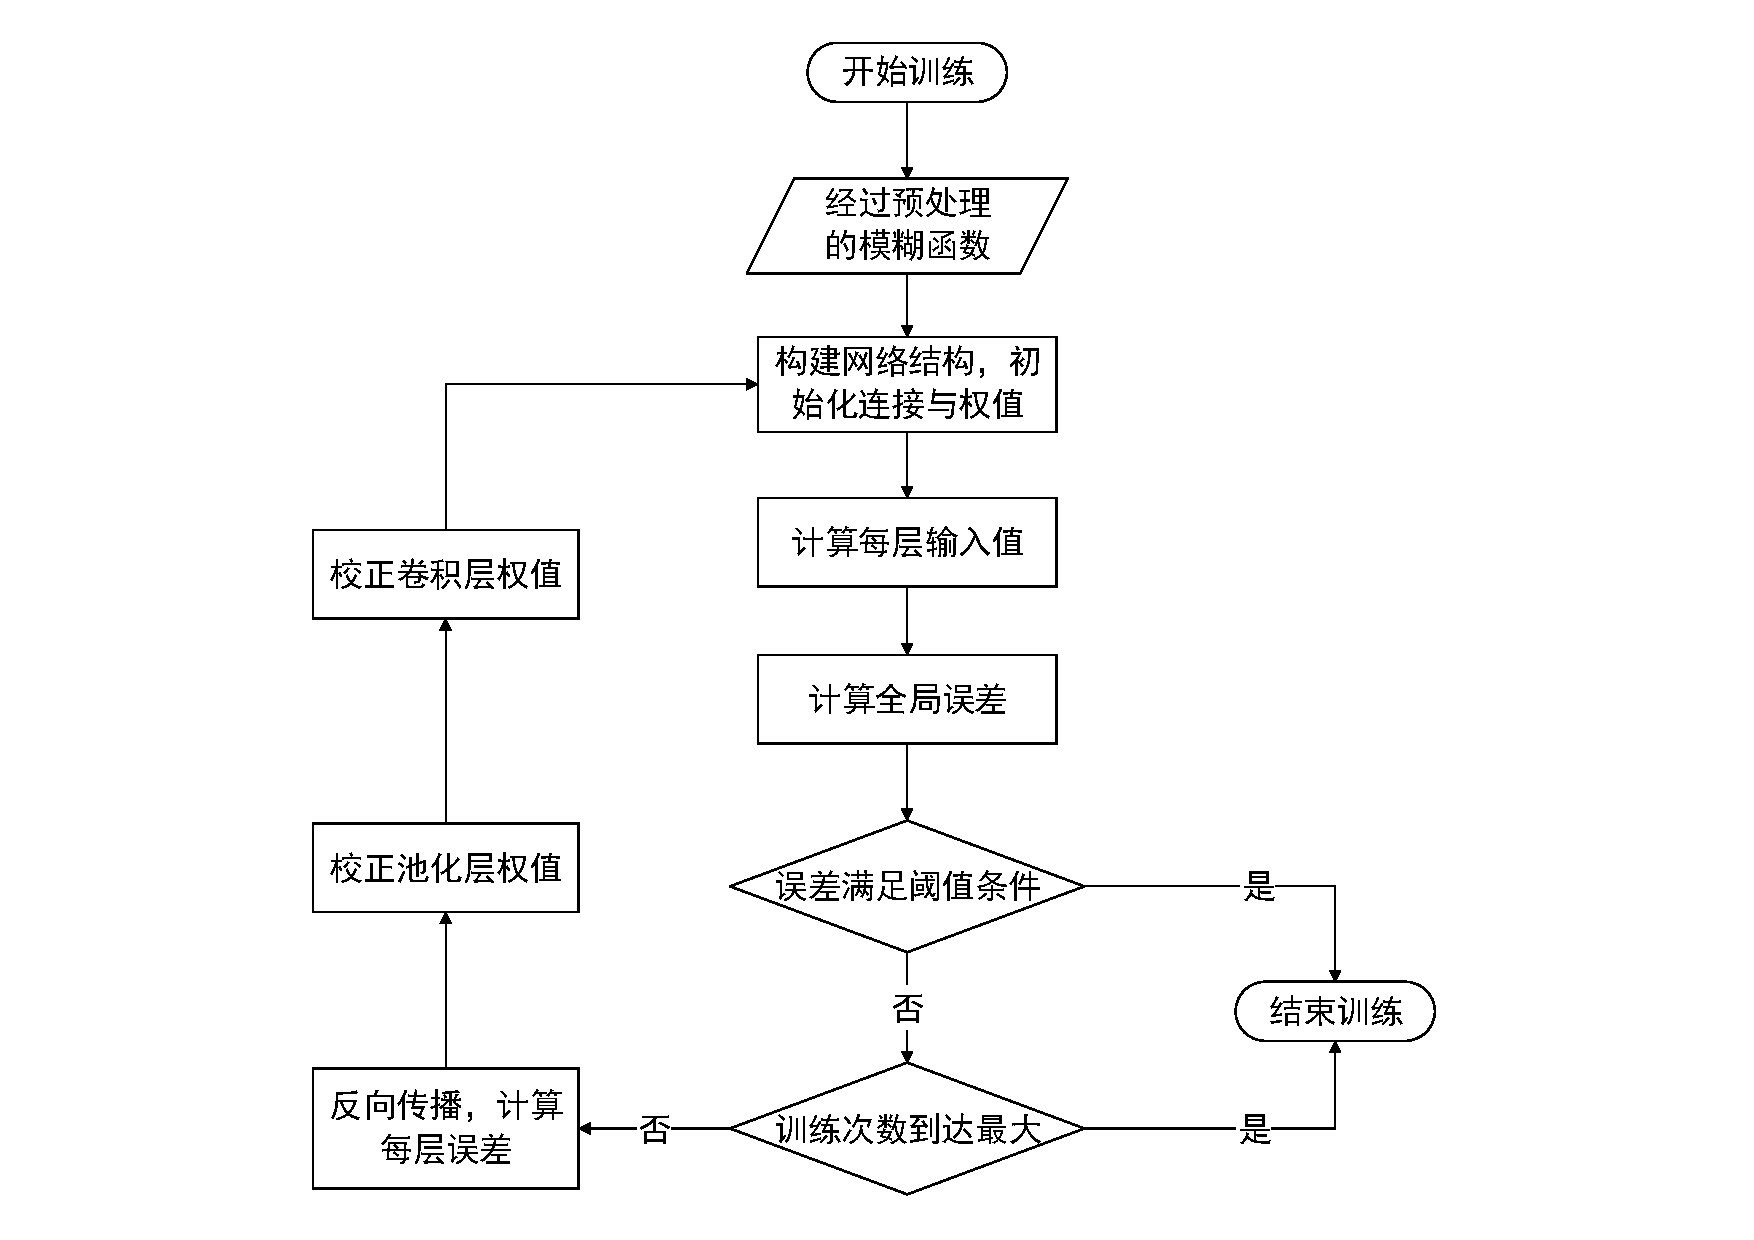
\includegraphics{figures/cnn_flow.pdf}
	\caption{深度卷积神经网络算法流程图}
\end{figure}


\section{SVM meta-recognition 设计}

支持向量机是一种流行的分类方法,因为它们可以在不需要大量数据的情况下产生良好的结果。我们可以利用所有的目标数据和未知目标的数据来作为训练样本对该SVM分类器进行训练,本部分我们以深度卷积神经网络的输出作为该分类器的输入,利用各类别的概率作为其特征进行训练识别。由于在类别的识别过程中,存在一定的波动性,这个会影响对于是否属于未知类别的分类判断,我们这里选取对于来自同一个辐射源的连续10拍的识别结果进行一个平均作为最终的输入。

下面是对于SVM分类器的设计,首先是核函数的选择。核函数将输入空间映射到高维特征空间,最终在高维特征空间中构造出最优分离超平面,从而把平面上本身不好分的非线性数据分开。常用的核函数为线性核函数和高斯核函数。对于核函数的选择,一般分为三种情况:

\begin{itemize}
	\item  Feature的数量很大,跟样本数量差不多,这时候选用LR或者是Linear Kernel的SVM
	\item  Feature的数量比较小,样本数量一般,不算大也不算小,选用SVM+Gaussian Kernel
	\item  Feature的数量比较小,而样本数量很多,需要手工添加一些feature变成第一种情况
\end{itemize}

由于我们的问题符合情况2,故选择高斯核函数。

支持向量机具有两个关键参数,惩罚参数$C$的和核参数$\sigma$,这两个参数的取值在很大程度上决定了SVM的性能的优劣。核函数的参数主要影响样本数据在高维特征空间中分布的复杂程度,即维数。特征子空间的维数越高,那么得到的最优分类超平面就会越复杂。反之亦然。因此只有选择合适的核参数得到合适的特征子空间,才能得到推广能力良好的SVM分类器。本文中用到的是高斯核参数。大量的实验数据表明,如果与样本点之间的距离很小,$\sigma\rightarrow0$;如果与样本点之间的距离很大时,$\sigma\rightarrow\infty$;当$\sigma$很小,高斯核函数支持向量机得到的判别函数差不多是一个常数,出现过拟合现象。当$\sigma$很大时,样本的正确分类率也会比较低。

惩罚参数是影响SVM算法性能的另一个重要因素。它的作用主要是调节特征子空间中SVM模型的置信范围与经验风险的比例,使支持向量机的泛化能力达到最好。特征子空间不同时,最优参数值取值也会不同。惩罚参数与经验误差的惩罚和SVM的复杂度成正比,与经验风险值成反比,反之亦然。因此,选择合适的惩罚参数也是非常重要的。

从上面的分析可以看出,核参数影响着映射函数、进而影响样本子空间的复杂度。最后会影响分类机性能的好坏。惩罚参数作用是在数据子空间中调节学习机器自信区间的范围。这些都说明了惩罚参数和核参数的选择非常重要。


\section{仿真实验与分析}


\subsection{实验环境}

由于我们原始获得的数据为IQ两路数据,为了更好的捕捉到回波的特征信息,我们对数据进行了一个变换,求取其模糊函数,并做偏移为0附件的一个切片。由于深度学习需要大量的数据进行训练学习,而本身数据量偏少,故我们在已有数据的基础上在一定信噪比的前提下,生成部分仿真数据。

对于数据的选择方面,我们从数据中选择出2至8个类别分别进行实验,对于每一个类别,我们均选择大约10000组数据,其中70\%作为训练样本,20\%作为交叉验证样本,10\%作为测试样本,同时在测试样本中又添加了与已知分类等数量的未知分类的数据进行测试。
\begin{figure}
	\centering
	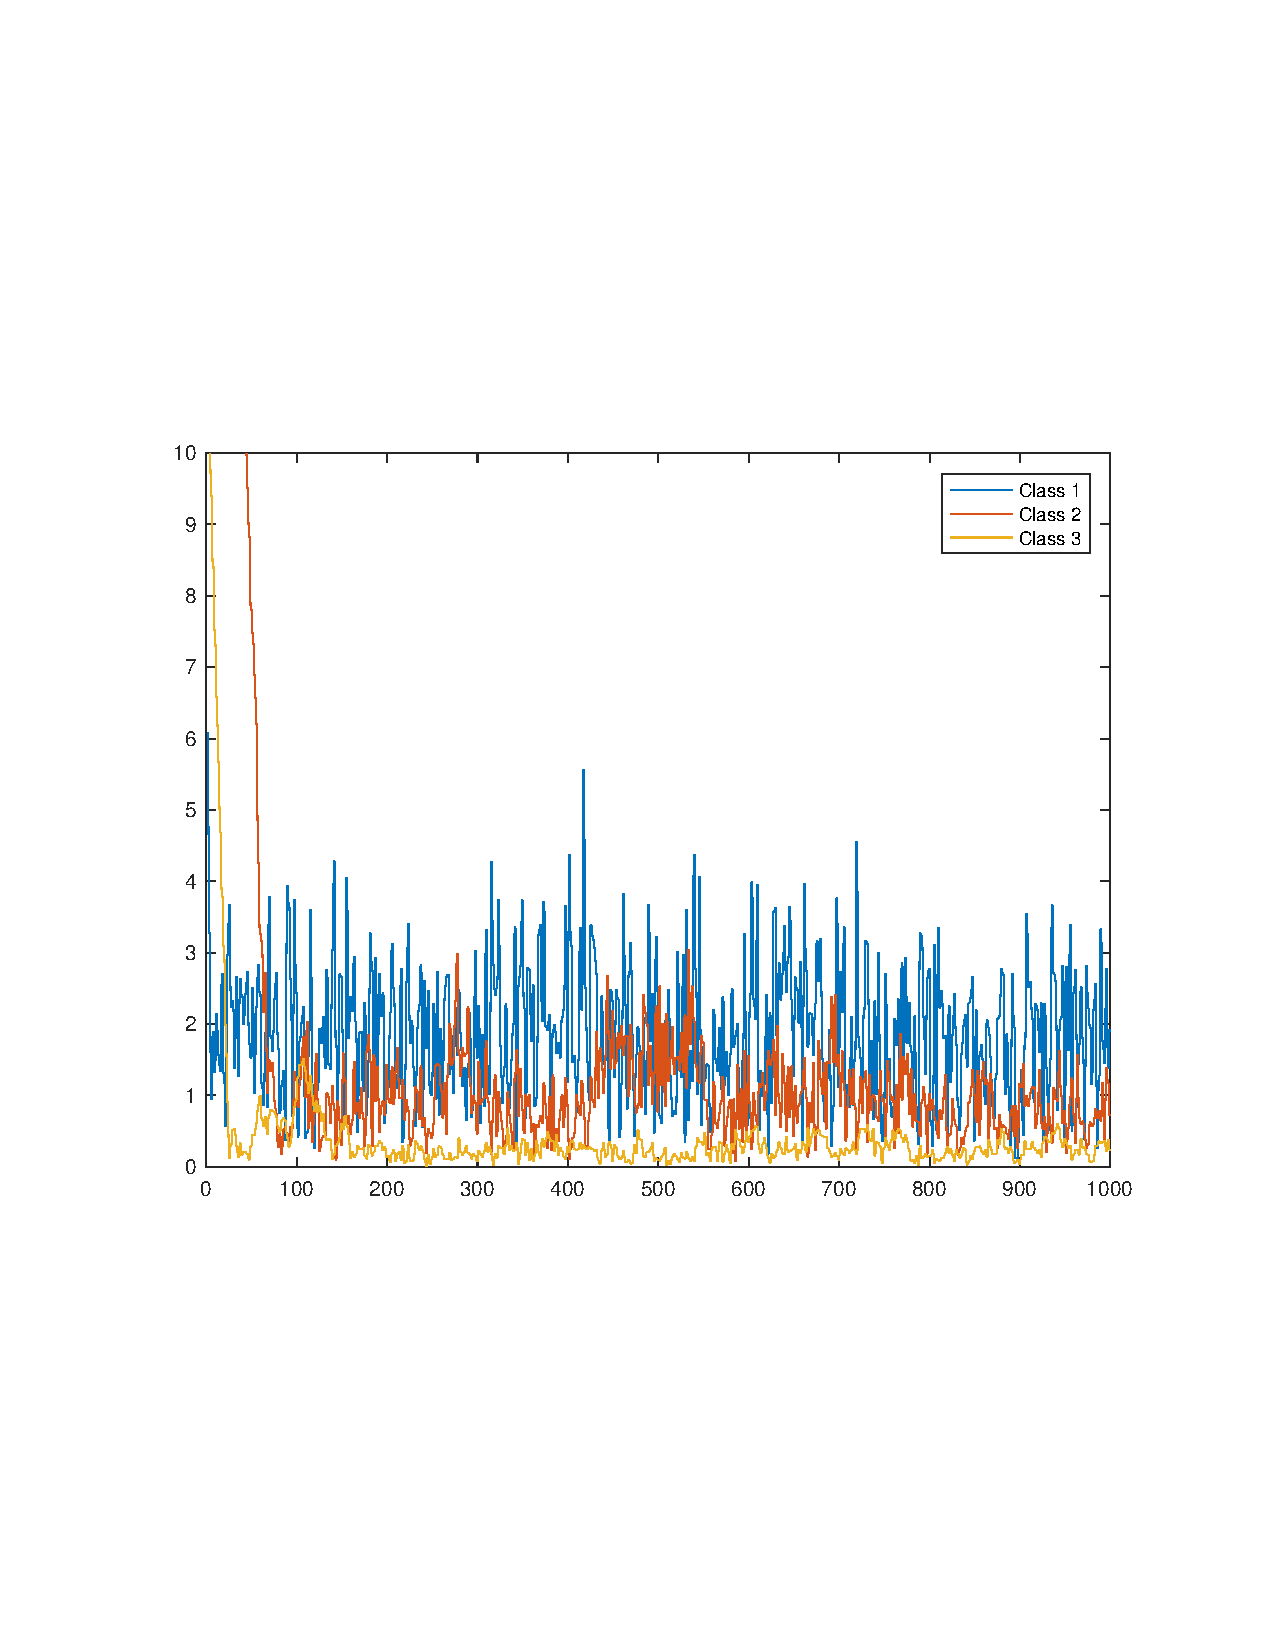
\includegraphics{figures/diff_data.pdf}
	\caption{不同类别样本特征图}
\end{figure}


由于该变换后,数据之间的差距比较大,我们对数据进行了归一化。我们采用的归一化方法为min-max标准化(Min-Max Normalization),也称为离差标准化,是对原始数据的线性变换,使结果值映射到[0 , 1]之间。转换函数如下:
\begin{equation}
x^{*}=\frac{x-x_{min}}{x_{max}-x_{min}}
\end{equation}
其中$x_{max}$为样本数据的最大值,$x_{min}$为样本数据的最小值。

我们采用网格搜索法对SVM参数进行调优,最终选择参数惩罚参数为32,核参数$\sigma$为0.0312。

\subsection{实验结果分析}

在上述样本的情形下,我们通过选取不同的类别数目,进行训练和测试得到下表的识别结果。从表中数据我们可以看出,随着样本类别数的增加,对于未知分类的识别准确率也随之有了大幅度的增加,而另一方面随着类别的增加,对于每个类别的识别准确率有一定的降低,但是仍然维持在比较高的水平。
\begin{figure}
	\centering
	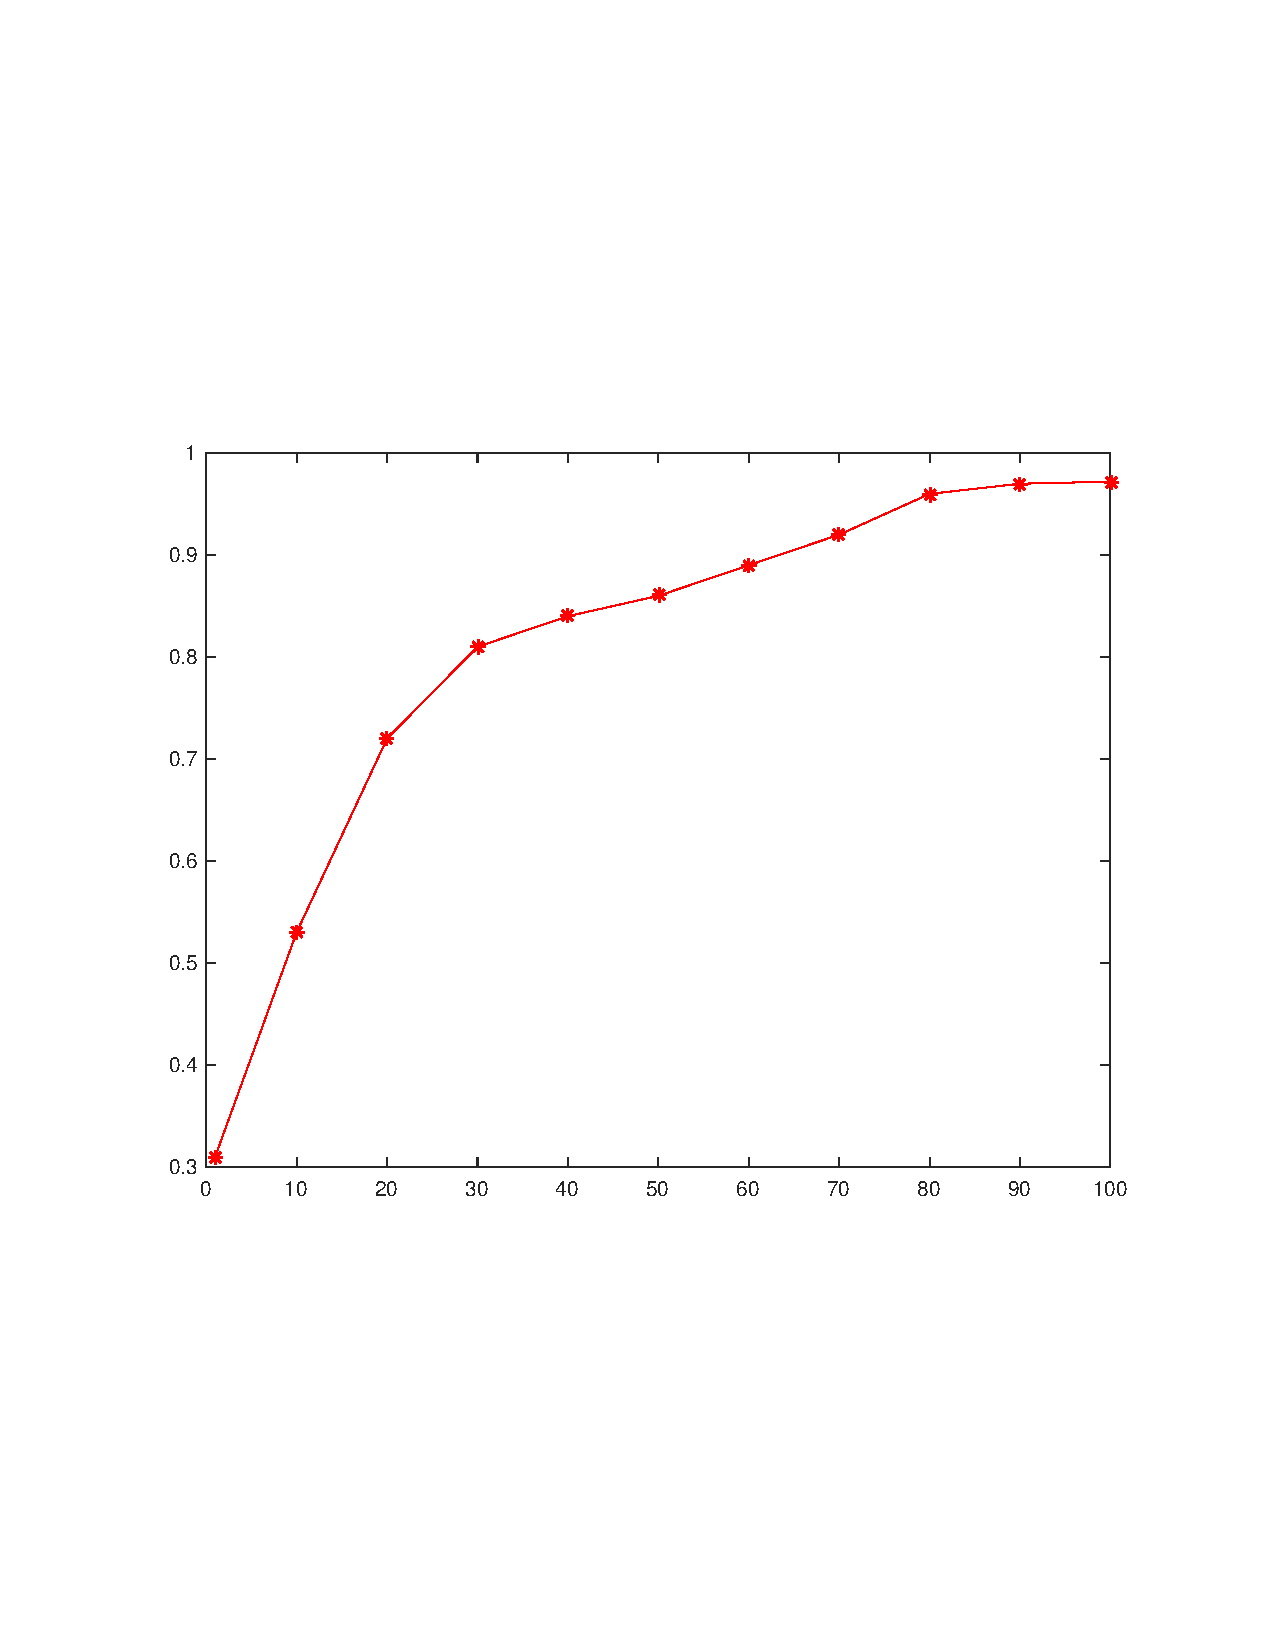
\includegraphics{figures/diff_epoch.pdf}
	\caption{迭代次数与识别准确率曲线图}
\end{figure}






\section{结束语}

本文针对复杂电磁环境下辐射源的识别面临的电磁信号干扰大、雷达信号参数相近等问题与挑战,利用深度学习的思想与方法,深入研究辐射源脉内细微特征,设计合适的神经网络结构,并基于实际机载气象雷达数据进行初步验证。主要特色与创新点如下:


(1)利用深度学习方法进行辐射源识别前沿。通过对现有辐射源信号进行分析,利用其脉内细微特征作为训练样本,使得识别准确率有了较大的进步。虽然已有研究利用神经网络、支持向量机等机器学习算法进行识别,但是仍然需要基于雷达信号的基本参数,没有考虑信号的内部特征参数。

(2)本文采用方法具有较强的抗噪声、抗干扰能力。传统方法进行辐射源个体识别前均需进行降噪、多径抑制和分选等复杂的信号预处理工作,这些操作会在一定程度上削弱雷达的个体特征。深度学习方法可以通过大量的样本,智能地判断各特征的权重,通过赋予不同的权重在保留雷达个体特征的情况下,避免干扰的影响。由此可见,本文所运用的方法具有较好的鲁棒性。

我们希望未来在目前的基础上,在下面几方面做进一步的研究:(1)利用更多的数据对算法进行进一步的验证,目前类别较少的情况下,部分结果会对选择的类别具有一定的依赖性,另一方面是选取更多更合适的特征进行训练学习;(2)利用集成学习提高学习精度;(3)尝试新方法对于未知分类识别;(4)对于未知分类,尝试利用无监督或者半监督学习进行训练学习。

%\begin{equation}
%  E=mc^2
%\end{equation}
%\begin{figure}
%  \centering
%  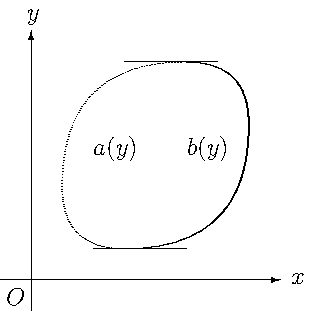
\includegraphics{figures/fig1-1.pdf}
%  \hskip 10pt
%  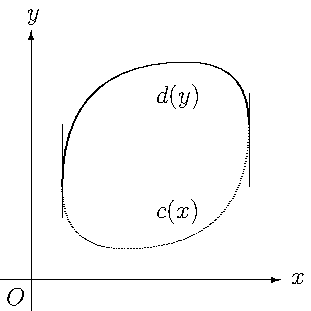
\includegraphics{figures/fig1-2.pdf}
%  \caption{测试图-区域}
%\end{figure}

%\begin{figure}
  %\centering
  %\includegraphics{figures/fig3.eps}
  %\caption{测试图-三维图}
%\end{figure}
%\begin{figure}
  %\centering
  %\includegraphics[width=0.3\textwidth]{figures/nwpu.jpg}
  %\caption{测试图-工大图标}
%\end{figure}
